\scanpage{110}
\deleted{Ceci posé, on prendra}

\[ \deleted{\tau=\{t',u',v'_1\},\quad \tau'=\{t',u_1,\unsure{v|w|v_1}\}} \]

\begin{center}---\end{center}
Changeons de notation donnés $a,s,t$ ($s,t$ liés à $a$, distincts et non liés) on complète triangles (distincts) $\{a,s,s'\}$, $\{a,t,t'\}$, on a triangle $\underline t_0$ de sommet $a$ distinct des $2$ précédents

% slanted
\margin{(Pour l'existence, \unsure{rapporter} la situation au triangle de base $\{a,s,s'\}$ -- il y a exactement \uline{$c$} choix \unsure{pour|de} $u$}

\figure{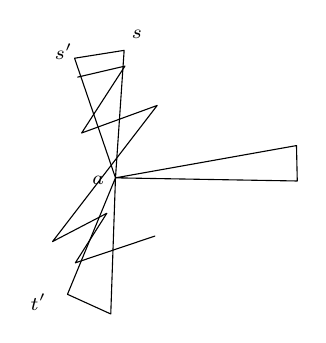
\begin{tikzpicture}[x=0.01cm,y=-0.01cm,line cap=round,line join=round]
\draw (263,757)--(211,605)--(274,595)--cycle;
\draw (263,757)--(493,716)--(494,761)--cycle;
\draw (263,757)--(202,905)--(257,930)--cycle;
\draw (215,629)--(275,615)--(220,700)--(316,665)--(183,838)--(252,802)--(212,865)--(313,831);

\node[inner sep=1pt,font=\scriptsize] at (197,597) {$s'$};
\node[inner sep=1pt,font=\scriptsize] at (290,575) {$s$};
\node[inner sep=1pt,font=\scriptsize] at (241,760) {$a$};
\node[inner sep=1pt,font=\scriptsize] at (165,915) {$t'$};
\end{tikzpicture}}

On choisit $u\neq a$ lié à $s$ et à $t$ (il est lié à un unique sommet de $\underline t_0$, qui est distinct de $a$, soit $b$), on prend $\{s,u,v\}\in T$, $\{t,u,w\}\in T$, \deleted{ils} \inserted{$v,w$} sont liés à $c$ (et sont distincts de $a,b$), on prend les triangles $\underline\sigma=\{c,v,v'\}$ et $\underline\tau=\{c,w,w'\}$, et on considère les symétries $\sigma_{\underline\sigma},\sigma_{\underline\tau}$, qui commutent (car $\underline\sigma,\underline\tau$ sont des triangles sécants).

\figure{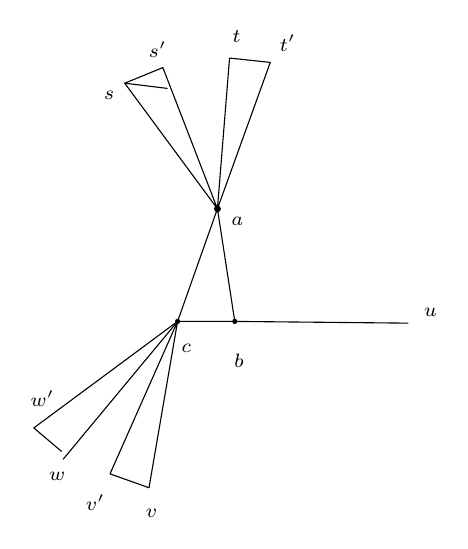
\begin{tikzpicture}[x=0.011cm,y=-0.011cm,line cap=round,line join=round]
\draw (237,1158)--(130,1013)--(174,995)--cycle;
\draw (130,1013)--(179,1019);
\draw (237,1158)--(251,984)--(298,989)--cycle;
\draw (237,1158)--(191,1288)--(257,1288)--cycle;
\draw (257,1288)--(457,1290);
\draw (191,1288)--(25,1411)--(57,1438);
\draw (191,1288)--(59,1447);
\draw (191,1288)--(113,1464)--(158,1480)--cycle;
\fill (237,1158) circle[radius=4];
\fill (191,1288) circle[radius=3];
\fill (257,1288) circle[radius=3];
\node[inner sep=1pt,font=\scriptsize] at (112,1027) {$s$};
\node[inner sep=1pt,font=\scriptsize] at (168,974) {$s'$};
\node[inner sep=1pt,font=\scriptsize] at (259,959) {$t$};
\node[inner sep=1pt,font=\scriptsize] at (318,967) {$t'$};
\node[inner sep=1pt,font=\scriptsize] at (260,1173) {$a$};
\node[inner sep=1pt,font=\scriptsize] at (201,1319) {$c$};
\node[inner sep=1pt,font=\scriptsize] at (262,1334) {$b$};
\node[inner sep=1pt,font=\scriptsize] at (483,1277) {$u$};
\node[inner sep=1pt,font=\scriptsize] at (35,1377) {$w'$};
\node[inner sep=1pt,font=\scriptsize] at (52,1467) {$w$};
\node[inner sep=1pt,font=\scriptsize] at (96,1497) {$v'$};
\node[inner sep=1pt,font=\scriptsize] at (161,1510) {$v$};
\end{tikzpicture}}

On a

\[
\begin{aligned}
\sigma_{\underline\sigma}s&=u &\text{car }\{s,u,v\}&\in T,\ v\in\underline\sigma\\
\sigma_{\underline\tau}u&=t &\text{car }\{t,u,w\}&\in T,\ w\in\unsure{\underline T|\underline\tau}
\end{aligned}
\]

% slanted
\margin{\deleted{\uline{NB} $\sigma_{\underline\sigma}u=s$ \quad $\sigma_{\underline\tau}s=u$ donc \deleted{\unsure{$s\leftrightarrow u$}} $Uu=\mathrm{id}$, \deleted{donc} \unsure{$U$ transforme|et transforme} $\{s,u,v\}\in\widetilde T$ en $\{t,u,w\}\in\widetilde T$}}

enfin, $\sigma_{\underline\sigma}$ et $\sigma_{\underline\tau}$ échangent $a$ et $b$ \inserted{et fixent $c$}, donc leur produit fixe les pts $a,b,c$. Donc $U=\sigma_{\underline\sigma}\,\sigma_{\underline\tau}$ transforme $(a,s)$ en $(a,t)$ et induit l'identité \deleted{sur} $(a,b,c)$

\deleted{\uline{NB} Supposons qu'on ait $r\in\widetilde E_c$ lié à $s$ et à $t$. Comme $s$ lié à $v$ (\deleted{\unsure{et|donc}} non à $v'$) $t$ lié à $w$ (donc non à $w'$), on a $r\neq v',w'$}

% archive sheet number: 109
